\begin{frame}{What is PastaQ?}

\begin{figure}[T]
  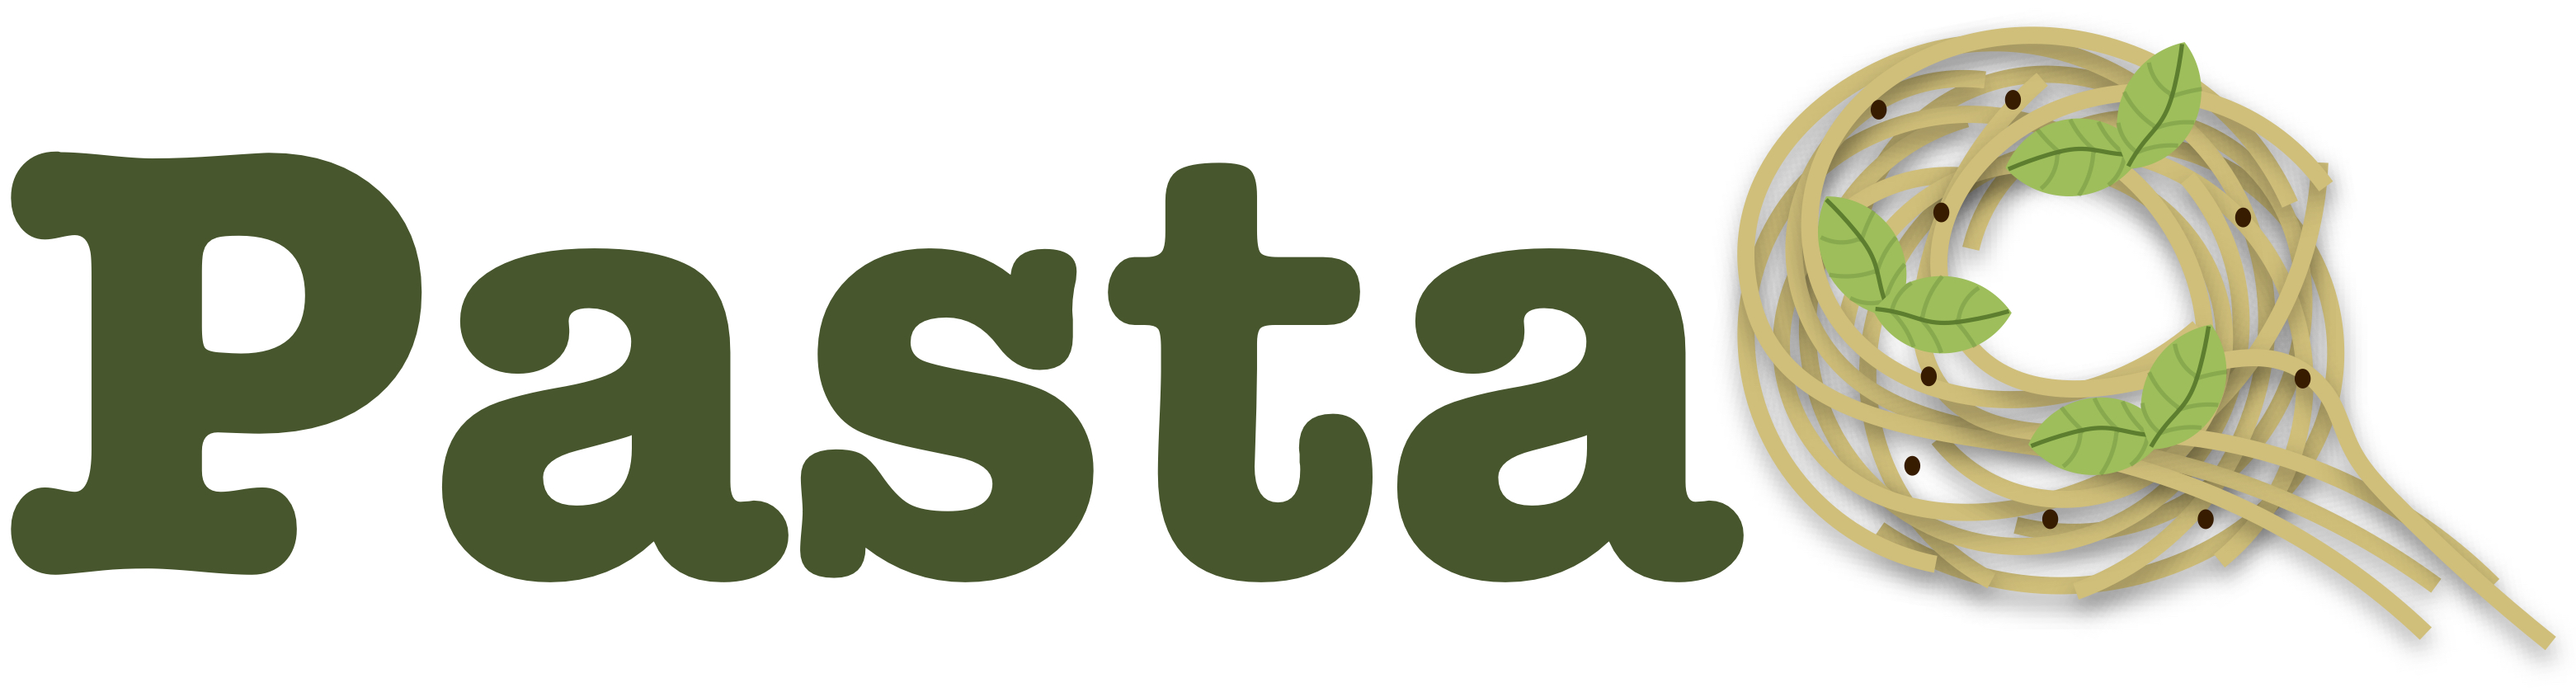
\includegraphics[width=0.5\textwidth]{
    slides/assets/what-is-pastaq-pastaq.jpg
  }
\end{figure}

\begin{columns}

  \setlength{\partopsep}{0pt}%

  \begin{column}[T]{0.65\textwidth}%

    \begin{itemize}[<+->]

      \item Initiated by \textbf{Giacomo Torlai} (AWS) while he was a postdoc at CCQ, co-developed by Giacomo and me.

    \end{itemize}

  \end{column}

  \begin{column}[T]{0.35\textwidth}%

    \vspace*{-0.4cm}

    \begin{figure}[T]
      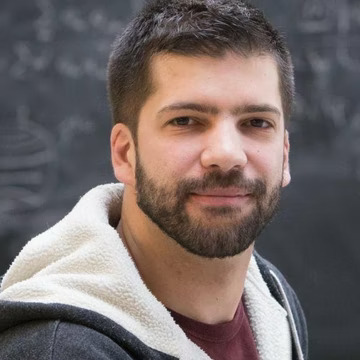
\includegraphics[width=0.5\textwidth]{
        slides/assets/what-is-pastaq-giacomo-torlai.jpg
      }
    \end{figure}

  \end{column}

\end{columns}

\begin{itemize}[<+->]

  \item Quantum computing extension to ITensor in Julia.

  \begin{itemize}[<+->]

    \item Tensor network-based quantum state and process tomography. 
    \item Extensive and customizable gate definitions.
    \item Built-in and easily extendable circuit definitions.
    \item Noisy circuit evolution with customizable noise models.
    \item Approximate circuit evolution and optimization with MPS/MPO, etc.

  \end{itemize}

  \item Find out more: \myhref{https://github.com/GTorlai/PastaQ.jl}{github.com/GTorlai/PastaQ.jl}

\end{itemize}

\end{frame}
